\documentclass{IEEEcsmag}

\usepackage[colorlinks,urlcolor=blue,linkcolor=blue,citecolor=blue]{hyperref}

\usepackage{upmath}

\jvol{XX}
\jnum{XX}
\paper{8}
\jmonth{May/June}
\jname{Computing in Science and Engineering}
\pubyear{2021}
\newtheorem{theorem}{Theorem}
\newtheorem{lemma}{Lemma}

\setcounter{secnumdepth}{0}

\begin{document}

\sptitle{Department: Head}
\editor{Editor: Name, xxxx@email}

\title{PyExaFMM: Designing a highly-performant particle fast multipole solver in Python with Numba}

\author{\ S. Kailasa}
\affil{\ Department of Mathematics, University College London}

\author{\ T. Betcke}
\affil{\ Department of Mathematics, University College London}

\author{\ T. Wang}
\affil{\ Department of Mechanical and Aerospace Engineering, The George Washington University}

\author{\ L. A. Barba}
\affil{\ Department of Mechanical and Aerospace Engineering, The George Washington University}

\markboth{Department Head}{Paper title}

\begin{abstract}
PyExaFMM is a pythonic kernel-independent particle fast multipole method [FMM] implementation, built on the success of the ExaFMM project, to answer the question of whether we could develop a highly-performant scientific code without resorting to a lower level language. The FMM is a good case study for understanding the maturity of Python for developing high-performance software, due its reliance on a complex heirarchical octree data structure. In this paper we offer an overview the kernel-independent FMM algorithm, and the key tool from Python's numerical ecosystem for developing high-performance applications, Numba. We also describe the mathematical and software development techniques we used to aid performance. We conclude by benchmarking the software's accuracy, speed, and memory footprint with respect to the state of the art C++ implementation from the ExaFMM project. We report that we are able to achieve runtimes within $\mathcal{O}(10)$ of the state of the art, with comparable accuracy for three dimensional electrostatic problems.

\end{abstract}

\maketitle

\chapterinitial{The Fast Multipole Method} [FMM], originally developed by Greengard and Rokhlin \cite{Greengard1987}, approximates the solution of the so called $N$ body problem, in which one seeks to calculate the pairwise interactions between $N$ objects. This problem arises in numerous contexts in physics and engineering. Consider the calculation of electrostatic potential, $\phi(x_j)$, for a given charged particle at position $x_j$, or `target', due to $N$ particles at positions $x_i$, or `sources', where $i \in [1, ..., N]$, each with a charge $q_i$,

\begin{eqnarray}
	\phi(x_j) = \sum_{i=1}^{N} K(x_i, x_j) q_i,
\label{eq:sec:intro:nbody_problem}
\end{eqnarray}

here $K(\cdot, \cdot)$ is called the Green's function, or kernel function, which for electrostatic problems in three dimensions is,

\begin{eqnarray}
	K(x, y) = \frac{1}{4\epsilon_0\pi|x-y|},
\label{eq:sec:intro:laplace_kernel}
\end{eqnarray}

where $\epsilon_0$ is the permittivity of free space. This kernel function is often referred to as the Laplace kernel.

% The reasoning behind this name is that (\ref{eq:sec:intro:nbody_problem}) with the Laplace kernel represents the discretized integral form of the Laplace equation,

% \begin{eqnarray}
% 	-\Delta \phi = \frac{q}{\epsilon_0},
% \end{eqnarray}

% which is itself derived from Gauss' law of electrostatics,

% \begin{eqnarray}
% 	-\nabla \cdot E = \frac{q}{\epsilon_0},
% \end{eqnarray}

% where the electric field $E$ is represented in terms of a scalar potential $E=\nabla \phi$.

Attempting to evaluate the sum in (\ref{eq:sec:intro:nbody_problem}) naively for $N$ target particles at positions $x_j$ where $j \in [1,...,N]$ due to $N$ sources, results in algorithm of $\mathcal{O}(N^2)$ runtime complexity, however the FMM is able to approximate (\ref{eq:sec:intro:nbody_problem}) with just $\mathcal{O}(N)$ runtime complexity, with proscribed error bounds.
The key idea behind the FMM is to encode the potential in the far field due to a cluster of particles with a representative analytic multipole expansion, which can be truncated to tune for desired accuracy. This truncation effectively allows for the user to approximate the sum in (\ref{eq:sec:intro:nbody_problem}) with fewer calculations. However, the coefficients of a given multipole expansion are kernel-dependent in the sense that they will depend on the form of (\ref{eq:sec:intro:laplace_kernel}). Originally introduced by Ying et. al \cite{Ying2004}, the kernel-independent fast multipole method [KIFMM] represents the multipole expansions due to a cluster of charges as set of equivalent densities supported on a surface enclosing the cluster, with the fields generated by the charges matched with the equivalent field via a least-squares fitting in the far field. This approach has the useful property of relying only on evaluations of the kernels, rather than analytic series expansions. This means that is can be programmed in a kernel-agnostic way and applied to a variety of problems. As originally developed in \cite{Ying2004}, the KIFMM generalizes the FMM to non-oscillatory second-order elliptic partial differential equations with constant coefficients, however further work has extended the method to include oscillatory problems \cite{Engquist2007}.

Python has emerged as the de-facto standard for the majority of computational scientists. It offers the ability to rapidly prototype

In this article we begin by providing an overview of the mathematical formulation behind the KIFMM, before introducing Numba and discussing how it is used by PyExaFMM to accelerate computations, as well as program efficient data structures. We continue, by discussing the mathematical and software based optimizations used by PyExaFMM for performance, and provide an overview of the software design used in order to implement optimizations effectively. We conclude with a discussion comparing the performance, in terms of accuracy, runtimes, and memory footprint, with the comparable state-of-the-art C++ implementation from the ExaFMM project, ExaFMM-T \cite{Wang2021}.

\section{THE KERNEL-INDEPENDENT FAST MULTIPOLE METHOD}

\subsection{Algorithm}

First introduced by Ying \cite{Ying2004}, the kernel-independent fast multipole method (KIFMM) \dots

\section{TECHNIQUES FOR ACHIEVING PERFORMANCE}

\subsection{What is Numba?}

What is does, how is it useful? Where do we use it, and why there. How much difference can it make in an idealized routine. What doesn't work, why doesn't it work. Where to be careful. Programming to an (invisible) framework \dots

Where is numba used heavily? Tree construction routines on Morton coordinates. Multithreading of tree construction, as well as P2M evaluation. Experiment to demonstrate the speed of kernel evaluation, with caveat that data must be pre-organised.

\subsection{Precomputing Operators}

Transfer vectors, hashing, HDF5, loading into memory.

\subsection{Compressing the M2L step with a randomised SVD}

Introduce \cite{Ying2004}. Numerical bounds on error out of scope, but show how experiments demonstrate that the FMM error dominates the SVD error.

\subsection{Software Architecture}

The key is separating routines to be accelerated, and organising data ready to run. The data organisation part (and it's slowness) should be demonstrated as a bottleneck using experiment.

\section{PERFORMANCE COMPARISON WITH STATE OF THE ART}

Description of main experiments, and how they are conducted. What are the main results? Are they expected from theory? What conclusions can be drawn about developing HPC codes entirely in Python, is it worth it?

\begin{figure}
\centerline{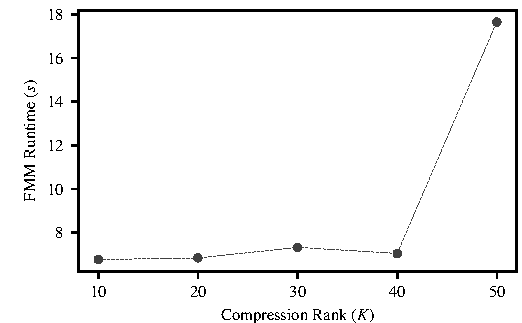
\includegraphics[width=18.5pc]{figures/compression_runtime.pdf}}
\caption{Compression Rank and runtime}
\end{figure}

\begin{figure}
\centerline{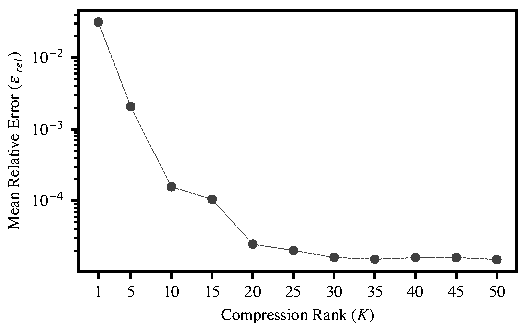
\includegraphics[width=18.5pc]{figures/compression_accuracy.pdf}}
\caption{Compression Rank and accuracy}
\end{figure}

% Larger figure
% \begin{figure*}
% \centerline{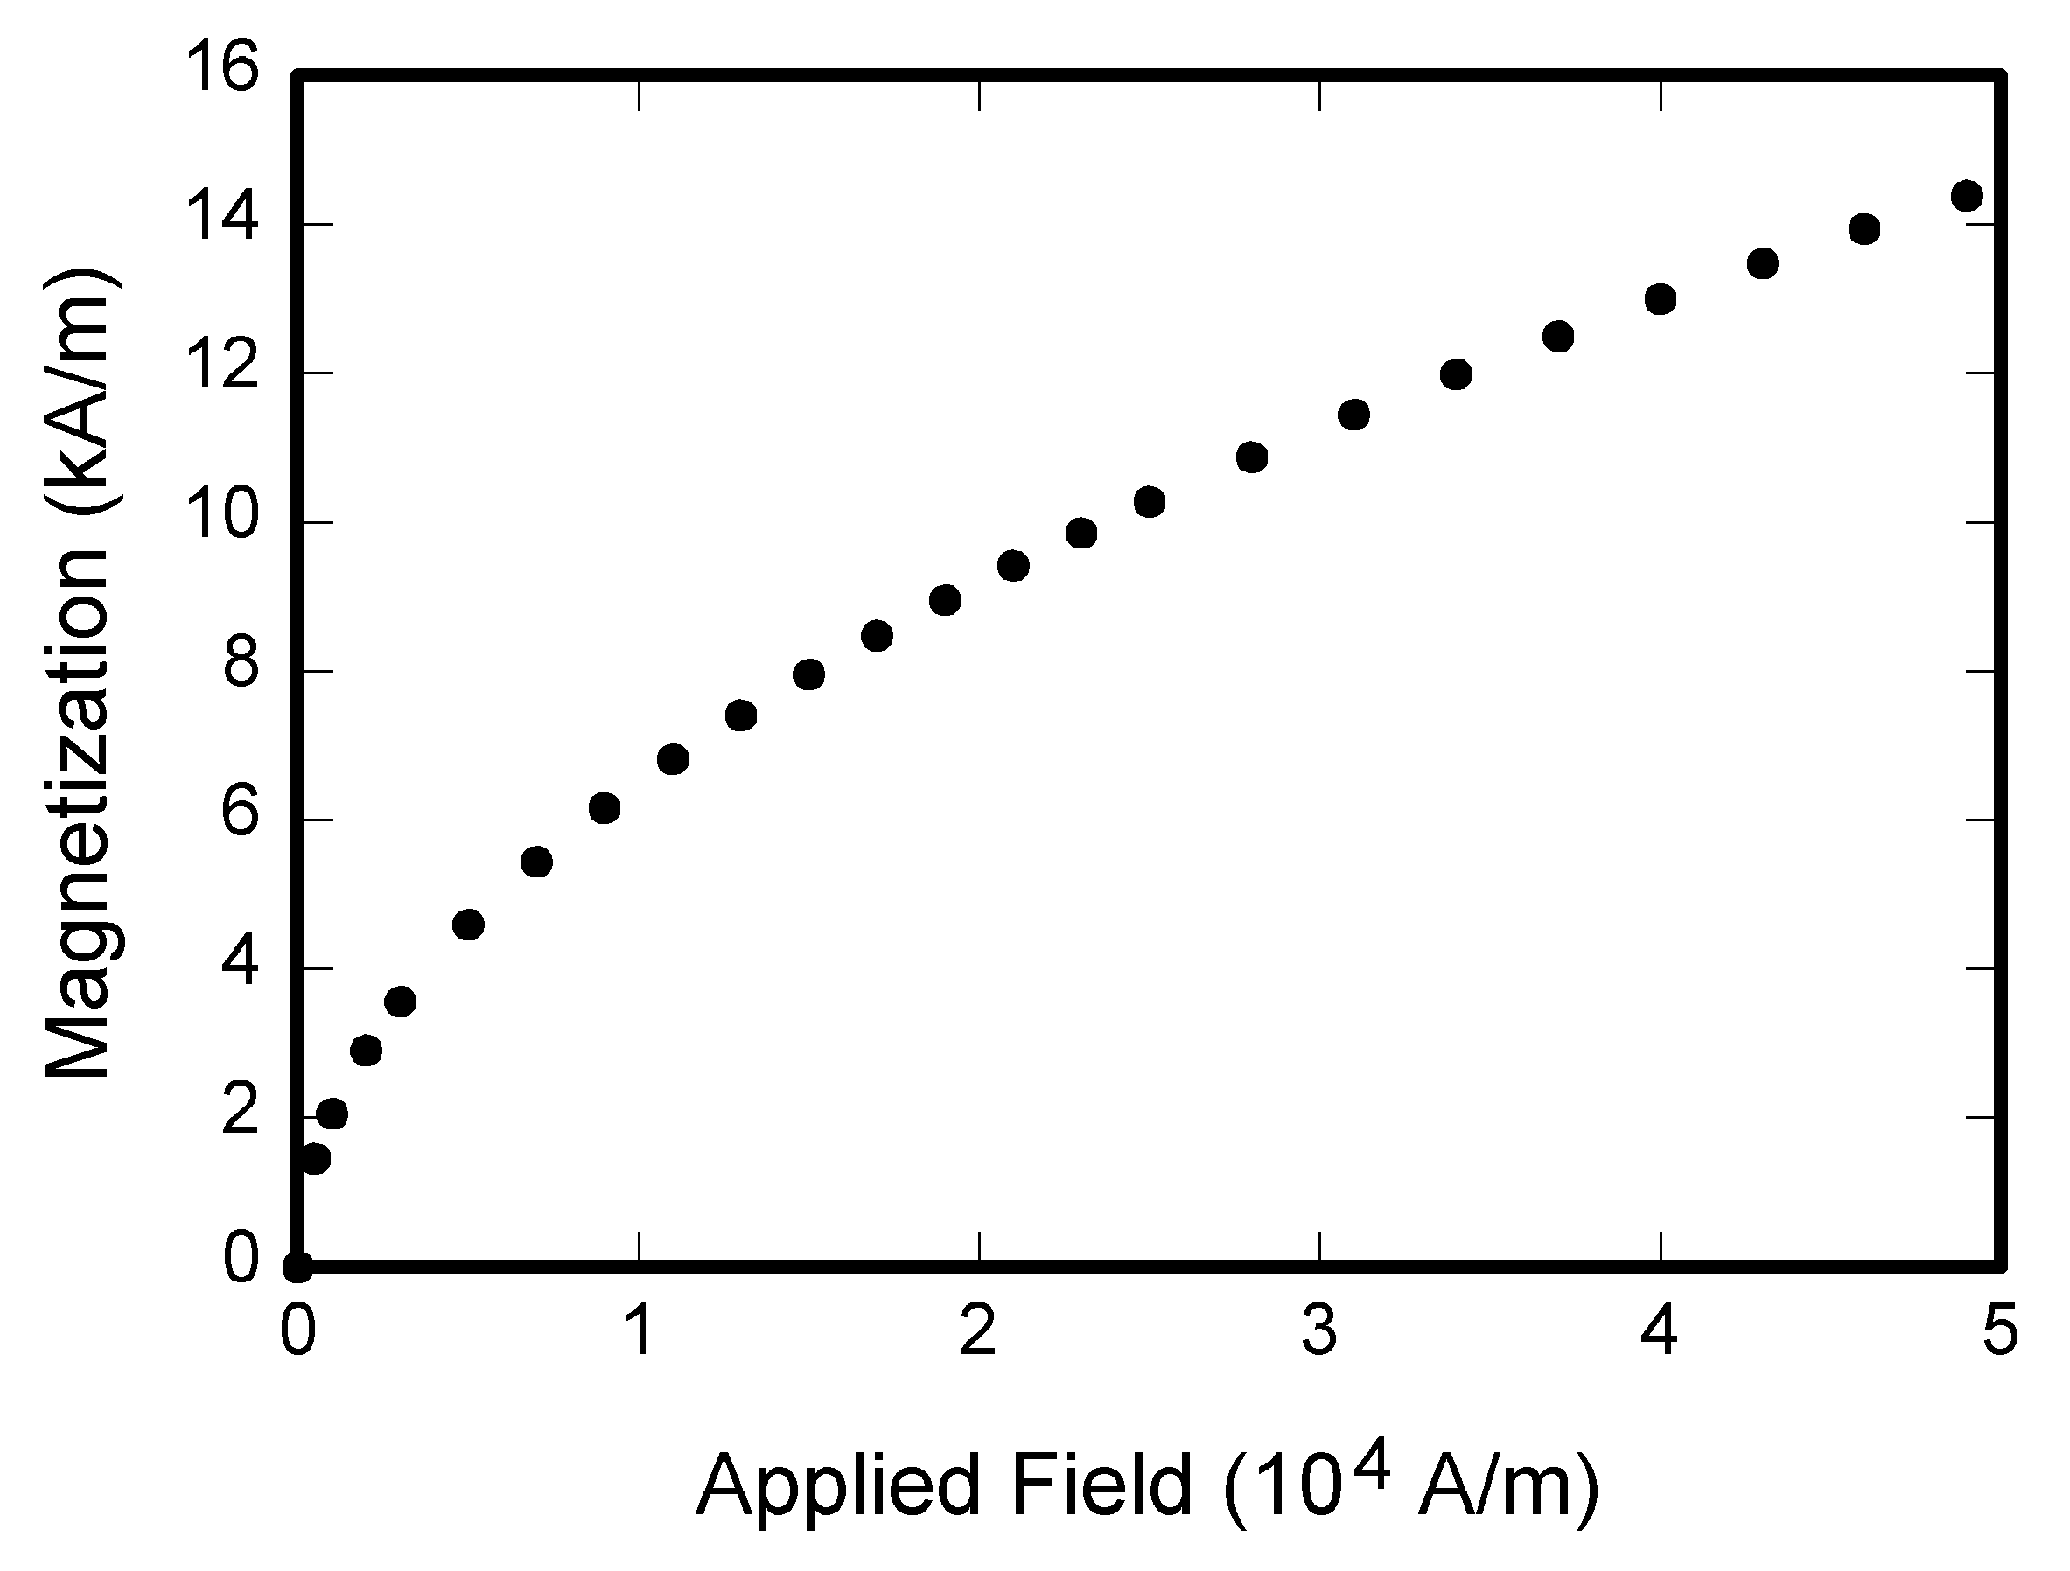
\includegraphics[width=26pc]{figures/fig1.png}}
% \caption{Note that ``Figure'' is spelled out. There is a period after the figure number, followed by one space. It is good practice to briefly explain the significance of the figure in the caption. (Used, with permission, from [4].)}
% \end{figure*}

% \begin{table}
% \caption{Units for magnetic properties.}
% \label{table}
% \small
% \begin{tabular*}{17.5pc}{@{}|p{29pt}|p{63pt}<{\raggedright}|p{80pt}<{\raggedright}|@{}}
% \hline
% Symbol&
% Quantity&
% Conversion from Gaussian and  CGS EMU to SI$^{\mathrm{a}}$ \\
% \hline
% $\Phi $&
% Magnetic flux&
% 1 Mx $\to  10^{-8}$ Wb $= 10^{-8}$ V $\cdot$ s \\
% $B$&
% Magnetic flux density,   magnetic induction&
% 1 G $\to  10^{-4}$ T $= 10^{-4}$ Wb/m$^{2}$ \\
% $H$&
% Magnetic field strength&
% 1 Oe $\to  10^{-3}/(4\pi )$ A/m \\
% $m$&
% Magnetic moment&
% 1 erg/G $=$ 1 emu   $\to 10^{-3}$ A $\cdot$ m$^{2} = 10^{-3}$ J/T \\
% $M$&
% Magnetization&
% 1 erg/(G $\cdot$ cm$^{3}) =$ 1 emu/cm$^{3}$   $\to 10^{-3}$ A/m \\
% 4$\pi M$&
% Magnetization&
% 1 G $\to  10^{-3}/(4\pi )$ A/m \\
% $\sigma $&
% Specific magnetization&
% 1 erg/(G $\cdot$ g) $=$ 1 emu/g $\to $ 1 A $\cdot$ m$^{2}$/kg \\
% $j$&
% Magnetic dipole   moment&
% 1 erg/G $=$ 1 emu   $\to 4\pi \times  10^{-10}$ Wb $\cdot$ m \\
% $J$&
% Magnetic polarization&
% 1 erg/(G $\cdot$ cm$^{3}) =$ 1 emu/cm$^{3}$  $\to 4\pi \times  10^{-4}$ T \\
% $\chi , \kappa $&
% Susceptibility&
% 1 $\to  4\pi $ \\
% $\chi_{\rho }$&
% Mass susceptibility&
% 1 cm$^{3}$/g $\to  4\pi \times  10^{-3}$ m$^{3}$/kg \\
% $\mu $&
% Permeability&
% 1 $\to  4\pi \times  10^{-7}$ H/m   $= 4\pi \times  10^{-7}$ Wb/(A $\cdot$ m) \\
% $\mu_{r}$&
% Relative permeability&
% $\mu \to \mu_{r}$ \\
% $w, W$&
% Energy density&
% 1 erg/cm$^{3} \to  10^{-1}$ J/m$^{3}$ \\
% $N, D$&
% Demagnetizing factor&
% 1 $\to  1/(4\pi )$ \\
% \hline
% \multicolumn{3}{@{}p{17.5pc}@{}}{Vertical lines are optional in tables. Statements that serve as captions for
% the entire table do not need footnote letters. }\\
% \multicolumn{3}{@{}p{17.5pc}@{}}{$^{\mathrm{a}}$Gaussian units are the same as cg emu for magnetostatics; Mx
% $=$ maxwell, G $=$ gauss, Oe $=$ oersted; Wb $=$ weber, V $=$ volt, s $=$
% second, T $=$ tesla, m $=$ meter, A $=$ ampere, J $=$ joule, kg $=$
% kilogram, H $=$ henry.}
% \end{tabular*}
% \label{tab1}
% \end{table}


\section{CONCLUSION}

What have we learned, what will we be working on next?

\section{ACKNOWLEDGMENT}

SK is supported by EPSRC Studentship 2417009.

\bibliography{pyexafmm}
\bibliographystyle{ieeetr}

\begin{IEEEbiography}{Srinath Kailasa}{\,} is a graduate student at University College London. He is currently pursuing a PhD in Computational Mathematics, having received an MPhys in Physics (2017) and an MSc Scientific Computing (2020) from the University of Durham, and University College London respectively. His research interests are in high-performance and scientific computing. Contact him at srinath.kailasa.18@ucl.ac.uk.
\end{IEEEbiography}

\begin{IEEEbiography}{Timo Betcke}{\,}is a Professor of Computational Mathematics at University College London. Contact him at t.betcke@ucl.ac.uk.
\end{IEEEbiography}

\begin{IEEEbiography}{Tingyu Wang}{\,}is a PhD student in Mechanical Engineering at the George Washington University. Contact him at twang66@email.gwu.edu.
\end{IEEEbiography}

\begin{IEEEbiography}{Lorena. A. Barba}{\,}is a Professor of Mechanical and Aerospace Engineering at the George Washington University.  Contact her at labarba@email.gwu.edu.
\end{IEEEbiography}

\end{document}

